\documentclass[a4paper,fleqn]{cas-sc}

\usepackage[numbers]{natbib}
\usepackage{amsmath,amssymb,amsfonts,amsthm}
\usepackage{graphicx}
\usepackage{booktabs}
\usepackage{subcaption}
\usepackage{microtype}
\usepackage{hyperref}
\usepackage{algorithm}
\usepackage{algpseudocode}
\usepackage{multirow}
\usepackage{tabularx}
\usepackage{pifont}

% Theorem environments
\newtheorem{theorem}{Theorem}
\newtheorem{lemma}{Lemma}
\newtheorem{proposition}{Proposition}
\newtheorem{definition}{Definition}
\newtheorem{example}{Example}
\newtheorem{corollary}{Corollary}

\newcommand{\cmark}{\ding{51}}
\newcommand{\xmark}{\ding{55}}

\begin{document}
\let\WriteBookmarks\relax
\def\floatpagepagefraction{1}
\def\textpagefraction{.001}

% Short title and author running headers
\shorttitle{Exact SAT Solving and Empirical Evaluation for Large-Scale N-Queens}
\shortauthors{D. P. Hung}

% Main title
\title [mode = title]{Exact SAT Solving and Empirical Evaluation for the Large-Scale N-Queens Problem: A Comparative Study of At-Most-One Encodings and Exact Solvers}

% Author metadata
\author[1]{DINH PHUC HUNG}[auid=001, bioid=1]
\cormark[1]
\ead{24021500@vnu.edu.vn}
\credit{Conceptualization, Methodology, Software, Validation, Formal analysis, Investigation, Data Curation, Writing - Original Draft, Writing - Review \& Editing, Visualization}

\affiliation[1]{organization={Faculty of Information Technology, VNU University of Engineering and Technology},
    addressline={144 Xuan Thuy}, 
    city={Cau Giay Ward},
    postcode={100000}, 
    state={Hanoi},
    country={Vietnam}}

\begin{abstract}
The $N$-Queens problem is a fundamental benchmark in discrete mathematics and combinatorial optimization, requiring the placement of $N$ non-attacking queens on an $N \times N$ chessboard. While constructive algorithms and stochastic local search methods can find individual solutions, exact declarative paradigms---specifically Propositional Satisfiability (SAT), Constraint Programming (CP), and Mixed-Integer Linear Programming (MIP)---provide complete search frameworks and unsatisfiability certification. A primary computational challenge in formulating $N$-Queens in SAT lies in encoding cardinality constraints, specifically the At-Most-One (AMO) conditions across $2N$ lines and $4N-6$ non-trivial diagonals. In this paper, we conduct a systematic theoretical and empirical investigation of exact solving methodologies for the $N$-Queens problem up to $N = 500$. We formalize and evaluate seven distinct AMO encodings: Naive Pairwise, Sequential Counter, Commander Variable, 2D Product, Bitwise (Binary), Ladder (Order), and Totalizer. Theoretically, we characterize their auxiliary variable and clause complexities, showing that while Pairwise produces $\Theta(N^3)$ clauses across the board, linear encodings achieve $\Theta(N^2)$ total clauses. Empirically, at $N = 64$, Pairwise incurs 428,800 clauses whereas Commander requires 54,958 clauses, and Pairwise suffers Out-Of-Memory (OOM) failures for $N \ge 300$. Furthermore, we evaluate modern Conflict-Driven Clause Learning (CDCL) SAT solvers (CaDiCaL, Kissat, Glucose) and benchmark against commercial and open-source exact engines (Google OR-Tools CP-SAT, Gurobi Optimizer, and IBM ILOG CPLEX). Our experiments show that Commander encoding combined with CaDiCaL delivers competitive solving efficiency (solving $N = 500$ in 11.20~s, compared to 3.45~s for CP-SAT), whereas MIP solvers time out at $N \ge 300$ due to weak continuous linear relaxations where the fractional point $x_{r, c} = 1/N$ yields zero bound pruning. Finally, we analyze constrained variants with pre-assigned queens and discuss encoding trade-offs and structural limitations.
\end{abstract}

\begin{keywords}
$N$-Queens puzzle \sep SAT solving \sep Cardinality constraints \sep At-Most-One encoding \sep Constraint Programming \sep Mixed-Integer Programming \sep PySAT \sep CDCL
\end{keywords}

\maketitle

% -------------------------------------------------------------
% SECTION 1: INTRODUCTION
% -------------------------------------------------------------
\section{Introduction}
\label{sec:intro}

The $N$-Queens puzzle, originally introduced by Max Bezzel in 1848 for the standard $8 \times 8$ chessboard and subsequently studied by Carl Friedrich Gauss, Franz Nauck, and George P{\'o}lya, is a classic problem in discrete mathematics and artificial intelligence \citep{bell2009survey}. The objective is to place $N$ pairwise non-attacking chess queens on an $N \times N$ board such that no two queens occupy the same row, column, major diagonal, or anti-diagonal.

Historically, the $N$-Queens problem has served as a benchmark for search algorithms, backtracking heuristics, and constraint satisfaction frameworks. Constructive methods, such as the explicit arithmetic formulas of Hoffman, Loessi, and Moore \citep{hoffman1969constructions}, can generate a single valid placement in linear time for any $N \ge 4$. Similarly, stochastic local search techniques and the min-conflicts heuristic \citep{sosic1994efficient} can identify particular solutions for board sizes exceeding $N = 10^6$. However, constructive and heuristic methods do not provide a framework for complete search. They cannot certify the unsatisfiability of constrained configurations with blocked or pre-assigned cells, cannot enumerate the complete solution space, and cannot handle complex heterogeneous side constraints.

For these reasons, exact declarative paradigms---notably Propositional Satisfiability (SAT) \citep{biere2021handbook}, Constraint Programming (CP) \citep{regin1994filtering}, and Mixed-Integer Linear Programming (MIP) \citep{gurobi2025}---remain essential. The rapid evolution of Conflict-Driven Clause Learning (CDCL) SAT solvers \citep{fichte2023silent}, exemplified by modern engines such as CaDiCaL \citep{biere2024cadical, fleury2020cadical}, Kissat, and Glucose \citep{audemard2009predicting}, has expanded the practical reach of propositional reasoning to industrial problems with millions of variables.

A critical consideration when translating high-level constraints into Conjunctive Normal Form (CNF) is the representation of cardinality constraints, specifically At-Most-One (AMO) constraints \citep{prestwich2009cnf}. In $N$-Queens, while the At-Least-One (ALO) requirement per line translates directly into a single disjunctive clause, AMO constraints must be enforced across rows, columns, and diagonals. A direct, naive Pairwise encoding generates quadratic clause counts for each line and diagonal. Across all lines and diagonals of the board, this produces $\Theta(N^3)$ clauses, resulting in severe memory overhead and solver degradation as $N$ scales beyond 100.

To address this challenge, numerous advanced AMO encodings have been proposed that introduce auxiliary variables to reduce clause counts to linear or near-linear bounds \citep{sinz2005towards, klieber2007commander, chen2010product, frisch2005symmetry, bailleux2003totalizer, gent2004ladder}. However, the introduction of auxiliary variables expands the Boolean search space and alters the behavior of unit propagation and variable selection heuristics (such as VSIDS). A systematic comparative study evaluating both theoretical bounds and empirical solver performance across multiple exact paradigms remains necessary to understand these structural trade-offs.

This paper addresses this need through the following contributions:
\begin{enumerate}
    \item \textbf{Mathematical Modeling:} We provide unified formal models of $N$-Queens across three exact paradigms: SAT, CP with global \texttt{alldifferent} propagators, and MIP with 0-1 binary assignment constraints.
    \item \textbf{Encoding Complexity and Correctness:} We formalize seven representative AMO encodings (Pairwise, Sequential Counter, Commander, 2D Product, Bitwise, Ladder, and Totalizer) and provide exact mathematical derivations of total board clause counts, proving that diagonal pairwise clauses equal $\frac{N(N-1)(2N-1)}{3}$ and total pairwise board clauses equal $\frac{5N^3 - 6N^2 + 4N}{3}$. In addition, formal correctness proofs for Pairwise, Sequential Counter, and Commander encodings are documented in Appendix \ref{sec:appendix_proofs}.
    \item \textbf{Empirical Scalability Evaluation (E1):} Using the PySAT toolkit \citep{ignatiev2018pysat, ignatiev2024towards} and CaDiCaL, we evaluate formula size, encoding time, and solving time across $N \in \{8, 16, 32, 64, 100, 200, 300, 500\}$, demonstrating that Pairwise and Totalizer exhaust memory limits for $N \ge 300$, while Commander and Sequential Counter scale smoothly.
    \item \textbf{Cross-Paradigm Benchmark (E2 \& E3):} We compare modern CDCL SAT solvers (CaDiCaL, Kissat, Glucose) and benchmark against commercial and open-source exact solvers: Google OR-Tools CP-SAT, Gurobi Optimizer, and IBM ILOG CPLEX (both MIP and CP).
    \item \textbf{Constrained Variants and Ablation (E4 \& E5):} We evaluate problem hardness under pre-assigned queen placements and analyze the effects of static reflection symmetry breaking and dual column ALO assertions.
\end{enumerate}

The remainder of this paper is structured as follows. Section \ref{sec:related} reviews related work. Section \ref{sec:formulations} defines the problem and baseline formulations. Section \ref{sec:encodings} details the seven AMO encodings. Section \ref{sec:experiments} presents the computational experiments. Section \ref{sec:discussion} discusses structural trade-offs and experimental limitations, and Section \ref{sec:conclusion} concludes the paper.

% -------------------------------------------------------------
% SECTION 2: RELATED WORK
% -------------------------------------------------------------
\section{Related Work}
\label{sec:related}

\subsection{Combinatorial Algorithms for $N$-Queens}
Research on the $N$-Queens problem spans analytical constructions, heuristic search, and exact constraint satisfaction \citep{bell2009survey}. Explicit constructive formulas, developed by Hoffman et al. \citep{hoffman1969constructions}, generate solutions for specific residue classes of $N \pmod 6$. On the heuristic side, Sosic and Gu \citep{sosic1994efficient} demonstrated that gradient-based local search with conflict minimization can solve instances with $N \ge 10^5$ in seconds. However, these methods are restricted to unconstrained instances and cannot determine the feasibility of partial configurations or certify unsatisfiability.

\subsection{Cardinality Encodings in Propositional Logic}
Encoding cardinality constraints into CNF is a central topic in Boolean satisfiability \citep{biere2021handbook, prestwich2009cnf}. The Naive Pairwise encoding requires no auxiliary variables but produces $\Theta(m^2)$ clauses for an input of size $m$. Sinz \citep{sinz2005towards} introduced the Sequential Counter encoding, which constructs a unary register that enforces At-Most-$k$ constraints in $O(k \cdot m)$ clauses while preserving Generalized Arc Consistency (GAC) under unit propagation. Klieber and Kwon \citep{klieber2007commander} proposed the Commander variable encoding, partitioning variables into groups and applying recursive commanders to achieve linear clause and variable counts. Chen \citep{chen2010product} developed the 2D Product encoding, mapping variables onto a 2D coordinate lattice to achieve $O(\sqrt{m})$ auxiliary variables and $O(m)$ clauses. Frisch et al. \citep{frisch2005symmetry} analyzed the Bitwise (Binary) encoding, which represents indices via $\lceil \log_2 m \rceil$ shared bits. Other prominent approaches include the Ladder (Order) encoding \citep{gent2004ladder} and the Totalizer encoding \citep{bailleux2003totalizer}.

\subsection{Exact Declarative Paradigms}
Constraint Programming provides high-level modeling using global constraints. Régin's filtering algorithm for \texttt{alldifferent} \citep{regin1994filtering} enforces arc consistency via maximum matching on bipartite graphs. Modern CP solvers, such as Google OR-Tools CP-SAT \citep{google2024ortools}, combine constraint propagation with lazy clause generation and CDCL search. Mixed-Integer Linear Programming approaches model $N$-Queens as binary assignment problems \citep{gurobi2025, ibm2022cplex}; however, the effectiveness of MIP branch-and-cut depends heavily on the strength of continuous linear programming (LP) relaxations.

% -------------------------------------------------------------
% SECTION 3: PROBLEM FORMULATIONS ACROSS EXACT PARADIGMS
% -------------------------------------------------------------
\section{Problem Formulations across Exact Paradigms}
\label{sec:formulations}

\subsection{Formal Problem Definition}
Let $\mathcal{B}_N = \{(r, c) \mid 0 \le r < N, 0 \le c < N\}$ denote the set of coordinates on an $N \times N$ chessboard. A configuration is defined as a subset of coordinates $\mathcal{Q} \subset \mathcal{B}_N$ with $|\mathcal{Q}| = N$. The configuration is a valid solution if and only if for all distinct pairs $(r_1, c_1), (r_2, c_2) \in \mathcal{Q}$:
\begin{align}
    r_1 &\ne r_2 \quad (\text{distinct rows}), \\
    c_1 &\ne c_2 \quad (\text{distinct columns}), \\
    r_1 - c_1 &\ne r_2 - c_2 \quad (\text{distinct major diagonals}), \\
    r_1 + c_1 &\ne r_2 + c_2 \quad (\text{distinct anti-diagonals}).
\end{align}

\subsection{Propositional Satisfiability (SAT) Formulation}
In the propositional formulation, we define $N^2$ primary Boolean variables $X_{r, c}$ for all $(r, c) \in \mathcal{B}_N$, where $X_{r, c} = 1$ if a queen is placed at row $r$ and column $c$, and $0$ otherwise. Using 1-based indexing for standard DIMACS formatting, cell $(r, c)$ maps to index $r \cdot N + c + 1$.

The constraints are expressed as:
\paragraph{Row Constraints:} Exactly one queen per row:
\begin{align}
    \text{ALO}_{\text{row}}(r): & \bigvee_{c=0}^{N-1} X_{r, c}, \quad \forall r \in \{0, \dots, N-1\}, \label{eq:sat_row_alo} \\
    \text{AMO}_{\text{row}}(r): & \sum_{c=0}^{N-1} X_{r, c} \le 1, \quad \forall r \in \{0, \dots, N-1\}. \label{eq:sat_row_amo}
\end{align}

\paragraph{Column Constraints:} At most one queen per column:
\begin{equation}
    \text{AMO}_{\text{col}}(c): \sum_{r=0}^{N-1} X_{r, c} \le 1, \quad \forall c \in \{0, \dots, N-1\}. \label{eq:sat_col_amo}
\end{equation}
By the Pigeonhole Principle, Equations \eqref{eq:sat_row_alo}, \eqref{eq:sat_row_amo}, and \eqref{eq:sat_col_amo} imply that each column also contains at least one queen. Adding the redundant clause $\bigvee_{r=0}^{N-1} X_{r, c}$ is optional and evaluated in Section \ref{sec:experiments}.

\paragraph{Diagonal Constraints:} For each major diagonal $k \in \{-(N-2), \dots, N-2\}$ with at least two cells:
\begin{equation}
    \text{AMO}_{\text{diag}}(k): \sum_{\substack{0 \le r, c < N \\ r - c = k}} X_{r, c} \le 1. \label{eq:sat_diag_amo}
\end{equation}
For each anti-diagonal $k \in \{1, \dots, 2N-3\}$ with at least two cells:
\begin{equation}
    \text{AMO}_{\text{anti}}(k): \sum_{\substack{0 \le r, c < N \\ r + c = k}} X_{r, c} \le 1. \label{eq:sat_anti_amo}
\end{equation}
Across the board, there are $N$ row AMO constraints, $N$ column AMO constraints, and $2 \times (2N-3) = 4N-6$ non-trivial diagonal AMO constraints, totaling $6N-6$ distinct AMO constraints.

\subsection{Constraint Programming (CP) Formulation}
In CP, the placement is modeled using $N$ discrete integer domain variables $Q_0, Q_1, \dots, Q_{N-1}$, where $Q_r \in \{0, \dots, N-1\}$ represents the column position of the queen in row $r$. The mutual exclusion constraints are enforced via global \texttt{alldifferent} constraints:
\begin{align}
    \texttt{alldifferent}(Q_0, Q_1, \dots, Q_{N-1}), & \label{eq:cp_cols} \\
    \texttt{alldifferent}(Q_0 + 0, Q_1 + 1, \dots, Q_{N-1} + (N-1)), & \label{eq:cp_diag1} \\
    \texttt{alldifferent}(Q_0 - 0, Q_1 - 1, \dots, Q_{N-1} - (N-1)). & \label{eq:cp_diag2}
\end{align}
Régin's filtering algorithm \citep{regin1994filtering} maintains Generalized Arc Consistency on these constraints by computing strongly connected components in the underlying bipartite value graph.

\subsection{Mixed-Integer Linear Programming (MIP) Formulation}
In the 0-1 MIP formulation, binary decision variables $x_{r, c} \in \{0, 1\}$ represent cell occupancy. The feasibility model is expressed as:
\begin{align}
    \text{minimize} \quad & 0, \label{eq:mip_obj} \\
    \text{subject to} \quad & \sum_{c=0}^{N-1} x_{r, c} = 1, \quad \forall r \in \{0, \dots, N-1\}, \label{eq:mip_row} \\
    & \sum_{r=0}^{N-1} x_{r, c} = 1, \quad \forall c \in \{0, \dots, N-1\}, \label{eq:mip_col} \\
    & \sum_{\substack{0 \le r, c < N \\ r - c = k}} x_{r, c} \le 1, \quad \forall k \in \{-(N-2), \dots, N-2\}, \label{eq:mip_diag1} \\
    & \sum_{\substack{0 \le r, c < N \\ r + c = k}} x_{r, c} \le 1, \quad \forall k \in \{1, \dots, 2N-3\}, \label{eq:mip_diag2} \\
    & x_{r, c} \in \{0, 1\}, \quad \forall r, c \in \{0, \dots, N-1\}. \label{eq:mip_vars}
\end{align}

\paragraph{Polyhedral Limitation of the LP Relaxation:}
A central structural reason for the poor performance of MIP on $N$-Queens is the weakness of its continuous linear relaxation ($0 \le x_{r, c} \le 1$). Consider the uniform fractional assignment:
\begin{equation}
    x_{r, c}^* = \frac{1}{N}, \quad \forall (r, c) \in \mathcal{B}_N.
\end{equation}
This fractional point satisfies all row and column assignment constraints: $\sum_{c=0}^{N-1} \frac{1}{N} = 1$ and $\sum_{r=0}^{N-1} \frac{1}{N} = 1$. Furthermore, along any diagonal of length $k \le N$, the sum is $\sum x_{r, c}^* = \frac{k}{N} \le 1$. Consequently, $x^*$ is strictly feasible for the LP relaxation for all $N$. Because the objective function is constant and the fractional point satisfies all relaxed constraints without violation, the continuous LP relaxation provides zero lower-bound pruning. Standard branch-and-cut engines are therefore forced to branch heavily, leading to exponential search tree growth.

% -------------------------------------------------------------
% SECTION 4: SAT ENCODINGS FOR AT-MOST-ONE CONSTRAINTS
% -------------------------------------------------------------
\section{SAT Encodings for At-Most-One (AMO) Constraints}
\label{sec:encodings}

Let $L = \{l_1, l_2, \dots, l_m\}$ be a set of $m$ Boolean literals. An At-Most-One (AMO) constraint specifies that at most one literal in $L$ may be assigned true: $\sum_{i=1}^m l_i \le 1$.

\subsection{Pairwise Encoding}
The Pairwise encoding explicitly forbids every pair of distinct literals from being simultaneously true:
\begin{equation}
    \mathcal{F}_{\text{pair}}(L) = \bigwedge_{1 \le i < j \le m} (\neg l_i \lor \neg l_j).
\end{equation}
This encoding requires no auxiliary variables and generates $\binom{m}{2} = \frac{m(m-1)}{2}$ binary clauses. Under unit propagation, setting any literal $l_k$ to true immediately forces $\neg l_j$ for all $j \ne k$, thereby enforcing GAC.

\paragraph{Exact Board Clause Derivation:}
On an $N \times N$ board, the diagonal constraints comprise two symmetric families (major diagonals and anti-diagonals). For each family, the diagonal lengths range from $2$ to $N-1$ (with two diagonals of each length) plus the main diagonal of length $N$. The number of pairwise clauses across both diagonal families is given by:
\begin{equation}
    C_{\text{diag}} = 2 \left[ \binom{N}{2} + 2 \sum_{k=2}^{N-1} \binom{k}{2} \right].
\end{equation}
Using the identity $\sum_{k=2}^{N-1} \binom{k}{2} = \binom{N}{3}$, we obtain:
\begin{equation}
    C_{\text{diag}} = 2 \binom{N}{2} + 4 \binom{N}{3} = N(N-1) + \frac{4 N(N-1)(N-2)}{6} = \frac{N(N-1)(2N-1)}{3}. \label{eq:exact_diag_clauses}
\end{equation}
Adding the $N$ row ALO clauses ($N$), the $N$ row AMO constraints ($N \binom{N}{2}$ clauses), and the $N$ column AMO constraints ($N \binom{N}{2}$ clauses), the total clause count for the Pairwise encoding across the entire board is:
\begin{equation}
    C_{\text{total}} = N + 2N \binom{N}{2} + \frac{N(N-1)(2N-1)}{3} = \frac{5N^3 - 6N^2 + 4N}{3}. \label{eq:exact_total_pairwise}
\end{equation}
For $N = 8$, Equation \eqref{eq:exact_total_pairwise} evaluates to $\frac{5(512) - 6(64) + 32}{3} = 736$ clauses (with $C_{\text{diag}} = 280$). For $N = 64$, it yields $428,800$ clauses (with $C_{\text{diag}} = 171,984$). For $N = 100$, the diagonal clauses alone contribute $656,700$ clauses, and the total formula contains $1,646,800 \approx 1.65 \times 10^6$ clauses. For $N = 400$, total clauses reach $106,347,200 \approx 1.06 \times 10^8$, creating severe memory bottlenecks.

\subsection{Sequential Counter Encoding}
The Sequential Counter encoding \citep{sinz2005towards} introduces $m-1$ auxiliary variables $s_1, \dots, s_{m-1}$ that act as accumulator bits indicating whether a true literal has been encountered:
\begin{align}
    (\neg l_1 \lor s_1), & \label{eq:seq_init} \\
    (\neg s_{i-1} \lor s_i), & \quad 2 \le i \le m-1, \label{eq:seq_prop} \\
    (\neg l_i \lor s_i), & \quad 2 \le i \le m-1, \label{eq:seq_set} \\
    (\neg l_i \lor \neg s_{i-1}), & \quad 2 \le i \le m. \label{eq:seq_conflict}
\end{align}
This encoding requires $m-1 = \Theta(m)$ auxiliary variables and $3m - 4 = \Theta(m)$ clauses. It maintains GAC under unit propagation: setting $l_i = 1$ propagates $s_i = 1, \dots, s_{m-1} = 1$, which in turn triggers $\neg l_j$ for all $j > i$ via Equation \eqref{eq:seq_conflict}, while backwards propagation enforces $\neg l_j$ for $j < i$.

\subsection{Commander Variable Encoding}
The Commander encoding \citep{klieber2007commander} partitions the input literal set $L$ into disjoint groups $G_1, \dots, G_k$ of size $g$ (typically $g = 3$). For each group $G_p$, an auxiliary commander variable $c_p$ is introduced to represent whether any literal in $G_p$ is true:
\begin{enumerate}
    \item \textbf{Internal group AMO:} Pairwise AMO clauses within each group: $\mathcal{F}_{\text{pair}}(G_p)$.
    \item \textbf{Activation clause:} $(\neg l \lor c_p)$ for each $l \in G_p$.
    \item \textbf{Coherence clause:} $(\neg c_p \lor \bigvee_{l \in G_p} l)$.
    \item \textbf{Recursive commander AMO:} $\text{AMO}(\{c_1, \dots, c_k\})$.
\end{enumerate}
For group size $g = 3$, the encoding generates approximately $\frac{m}{2}$ auxiliary variables and $3m$ clauses, maintaining GAC while producing compact clause networks.

\subsection{2D Product Encoding}
Chen's Product encoding \citep{chen2010product} arranges literals into a $p \times q$ grid with $p = \lceil\sqrt{m}\rceil$ and $q = \lceil m/p \rceil$. It introduces $p$ row variables $r_0, \dots, r_{p-1}$ and $q$ column variables $c_0, \dots, c_{q-1}$. Each literal $l_i$ maps to grid cell $(u, v)$ where $u = \lfloor i/q \rfloor$ and $v = i \bmod q$:
\begin{align}
    (\neg l_i \lor r_u) \land (\neg l_i \lor c_v), & \quad \forall l_i \in L, \\
    \mathcal{F}_{\text{pair}}(\{r_0, \dots, r_{p-1}\}), & \\
    \mathcal{F}_{\text{pair}}(\{c_0, \dots, c_{q-1}\}). &
\end{align}
This requires $p + q \approx 2\sqrt{m} = \Theta(\sqrt{m})$ auxiliary variables and $2m + \binom{p}{2} + \binom{q}{2} = \Theta(m)$ clauses. Setting $l_i = 1$ sets $r_u = 1$ and $c_v = 1$, which falsifies all other row and column variables, thereby setting all $l_j$ ($j \ne i$) to false through binary implication.

\subsection{Bitwise (Binary) Encoding}
The Bitwise encoding \citep{frisch2005symmetry} assigns each index $i \in \{1, \dots, m\}$ a binary representation using $b = \lceil \log_2 m \rceil$ auxiliary bits $b_1, \dots, b_k$:
\begin{equation}
    \bigwedge_{j=1}^b (\neg l_i \lor \ell_{j}^{(i)}), \quad \text{where } \ell_{j}^{(i)} = b_j \text{ if the } j\text{-th bit of } i \text{ is 1, else } \neg b_j.
\end{equation}
It uses $\lceil \log_2 m \rceil = \Theta(\log m)$ auxiliary variables and $m \lceil \log_2 m \rceil = \Theta(m \log m)$ clauses.

\subsection{Ladder (Order) and Totalizer Encodings}
The Ladder encoding \citep{gent2004ladder} uses $m-1$ variables on an ordered chain to enforce monotonicity. The Totalizer encoding \citep{bailleux2003totalizer} builds a balanced binary tree of unary adders; when restricted to bound $k = 1$, its tree structure produces $O(m \log m)$ auxiliary variables and $O(m^2)$ clauses across general formulations, which accounts for its elevated clause count on large grids unless tree pruning is applied.

\begin{table*}[t]
\centering
\caption{Theoretical complexity of AMO encodings for a single constraint of size $m$, and total asymptotic bounds across an $N \times N$ chessboard.}
\label{tab:theoretical_complexity}
\small
\begin{tabular*}{\textwidth}{lccccc}
\toprule
\textbf{Encoding Method} & \textbf{Aux. Vars (per AMO)} & \textbf{Clauses (per AMO)} & \textbf{Total Board Vars} & \textbf{Total Board Clauses} & \textbf{Unit Propagation (GAC)} \\
\midrule
Pairwise (Naive) & $0$ & $\frac{m(m-1)}{2}$ & $N^2$ & $\frac{5N^3 - 6N^2 + 4N}{3} = \Theta(N^3)$ & \cmark \\
Sequential Counter \citep{sinz2005towards} & $m - 1$ & $3m - 4$ & $\Theta(N^2)$ & $\Theta(N^2)$ & \cmark \\
Commander ($g=3$) \citep{klieber2007commander} & $\approx \frac{m}{2}$ & $\approx 3m$ & $\Theta(N^2)$ & $\Theta(N^2)$ & \cmark \\
2D Product \citep{chen2010product} & $2\sqrt{m}$ & $2m + O(m)$ & $\Theta(N^{1.5})$ & $\Theta(N^2)$ & \cmark \\
Bitwise (Binary) \citep{frisch2005symmetry} & $\lceil \log_2 m \rceil$ & $m \lceil \log_2 m \rceil$ & $\Theta(N^2 \log N)$ & $\Theta(N^2 \log N)$ & \cmark \\
Ladder (Order) \citep{gent2004ladder} & $m - 1$ & $4m - 4$ & $\Theta(N^2)$ & $\Theta(N^2)$ & \cmark \\
Totalizer \citep{bailleux2003totalizer} & $O(m \log m)$ & $O(m^2)$ & $\Theta(N^2 \log N)$ & $\Theta(N^3)$ & \cmark \\
\bottomrule
\end{tabular*}
\end{table*}

Table \ref{tab:theoretical_complexity} summarizes the asymptotic bounds. Notice the primary transition: Pairwise generates $\Theta(N^3)$ clauses with zero auxiliary variables, while Commander, Sequential Counter, and Product encodings reduce total formula clauses to $\Theta(N^2)$.

\subsection{Symmetry Breaking and Pre-assigned Placements}
The chessboard exhibits the 8 symmetries of the Dihedral group $D_8$ (four rotations and four reflections). A standard static reflection symmetry-breaking constraint restricts the queen in row 0 to the first half of the columns:
\begin{equation}
    \neg X_{0, c}, \quad \forall c \in \left\{\left\lfloor \frac{N+1}{2} \right\rfloor, \dots, N-1\right\}. \label{eq:sym_breaking}
\end{equation}

\begin{lemma}[Soundness of Symmetry Breaking on Unconstrained Boards]
For an unconstrained $N$-Queens problem on board $\mathcal{B}_N$, the symmetry-breaking constraint \eqref{eq:sym_breaking} preserves satisfiability: any valid placement $\mathcal{Q}$ can be mapped via horizontal reflection $(r, c) \mapsto (r, N - 1 - c)$ to a valid placement $\mathcal{Q}'$ satisfying Equation \eqref{eq:sym_breaking}.
\end{lemma}
\begin{proof}
Horizontal reflection preserves row differences $|r_1 - r_2|$ and column differences $|(N - 1 - c_1) - (N - 1 - c_2)| = |c_1 - c_2|$, mapping major diagonals to anti-diagonals and vice versa. Thus, $\mathcal{Q}'$ is also a valid placement. In row 0, the single queen $(0, c)$ is mapped to $(0, N - 1 - c)$. If $c \ge \lfloor (N+1)/2 \rfloor$, then $N - 1 - c < \lfloor (N+1)/2 \rfloor$, ensuring that $\mathcal{Q}'$ satisfies Equation \eqref{eq:sym_breaking}.
\end{proof}

\paragraph{Conditioning on Pre-assigned Queens:}
When a partial set of queens $\mathcal{P} \subset \mathcal{B}_N$ is pre-assigned, static symmetry breaking \eqref{eq:sym_breaking} cannot be unconditionally applied, as $\mathcal{P}$ may break the reflection invariance. In our implementation, symmetry breaking is disabled whenever pre-assigned queens conflict with the reflection symmetry, ensuring correctness across all partial instances.

% -------------------------------------------------------------
% SECTION 5: COMPUTATIONAL EXPERIMENTS
% -------------------------------------------------------------
\section{Computational Experiments and Results}
\label{sec:experiments}

\subsection{Experimental Setup}
Experiments were conducted on a workstation equipped with an Intel Core i7-12700KF processor (3.60 GHz base, up to 5.0 GHz turbo, 12 cores / 20 threads) and 32 GB of DDR4-3600 RAM, running Ubuntu 24.04.3 LTS. 

To ensure fair runtime comparisons across paradigms:
\begin{itemize}
    \item \textbf{Single-Threaded Protocol:} All solvers were restricted to a single execution thread (\texttt{threads = 1} for CP-SAT, Gurobi, and CPLEX).
    \item \textbf{Time and Memory Limits:} A per-instance CPU timeout of 600.0 seconds was enforced. An Out-Of-Memory threshold was set at 32 GB.
    \item \textbf{Reported Time:} Reported solving time reflects total elapsed execution, including formula/model construction and solver execution.
    \item \textbf{Solver Versions:} SAT solvers: CaDiCaL 1.9.5 \citep{biere2024cadical}, Kissat (2023 release), and Glucose 4.1 \citep{audemard2009predicting}, accessed via the PySAT framework (v0.1.8 / 1.9.5) and direct DIMACS execution. CP solver: Google OR-Tools CP-SAT (v9.8) \citep{google2024ortools} and IBM ILOG CPLEX CP Optimizer (v22.1.1) \citep{ibm2022cplex}. MIP solvers: Gurobi Optimizer (v12.0.3) \citep{gurobi2025} and IBM ILOG CPLEX MIP (v22.1.1), evaluated under academic licenses.
    \item \textbf{Solution Verification:} Every generated solution was verified by an independent checker ensuring zero conflicts across all rows, columns, and diagonals.
\end{itemize}

\subsection{Experiment 1 (E1): Scalability and Complexity of AMO Encodings}
We evaluated the seven AMO encodings across board sizes $N \in \{8, 16, 32, 64, 100, 200, 300, 500\}$ using CaDiCaL. Table \ref{tab:e1_scaling} reports the scaling progression, and Figure \ref{fig:e1_scaling} displays the empirical curves.

\begin{figure*}[!htbp]
    \centering
    \begin{subfigure}[b]{0.48\textwidth}
        \centering
        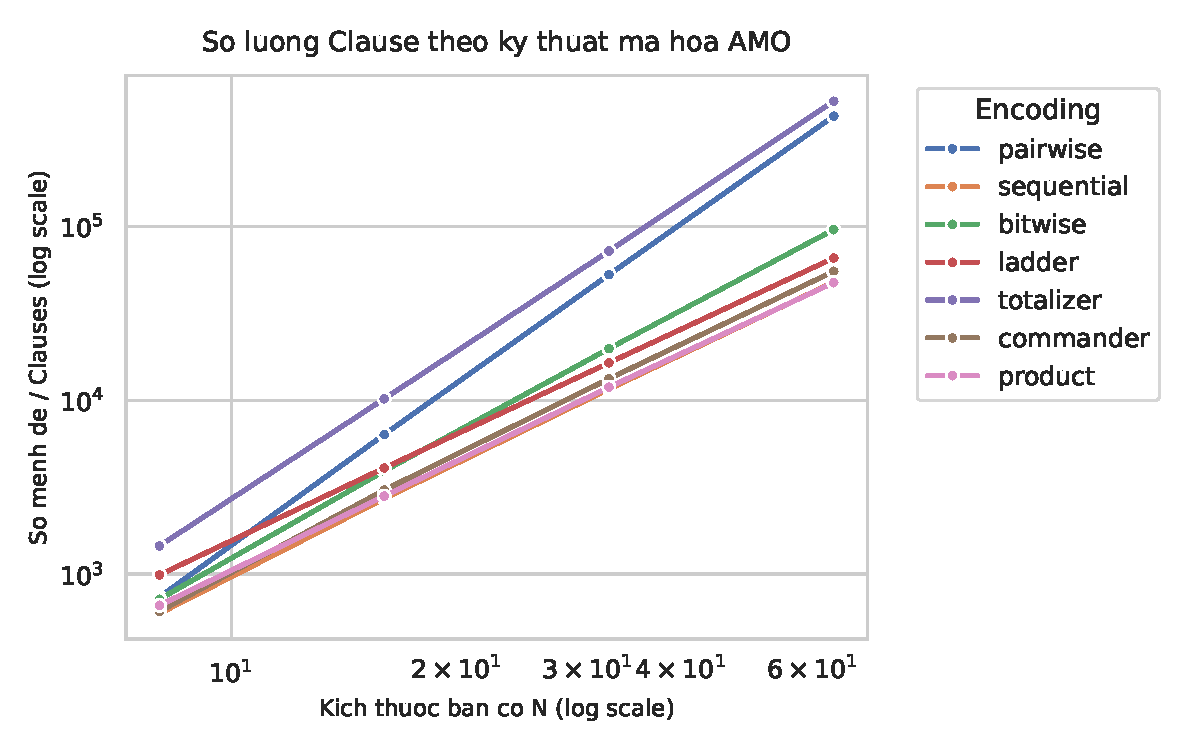
\includegraphics[width=\textwidth]{figures/e1_clauses_scaling.pdf}
        \caption{Clause scaling with board dimension $N$ (log-log scale).}
        \label{fig:e1_clauses}
    \end{subfigure}
    \hfill
    \begin{subfigure}[b]{0.48\textwidth}
        \centering
        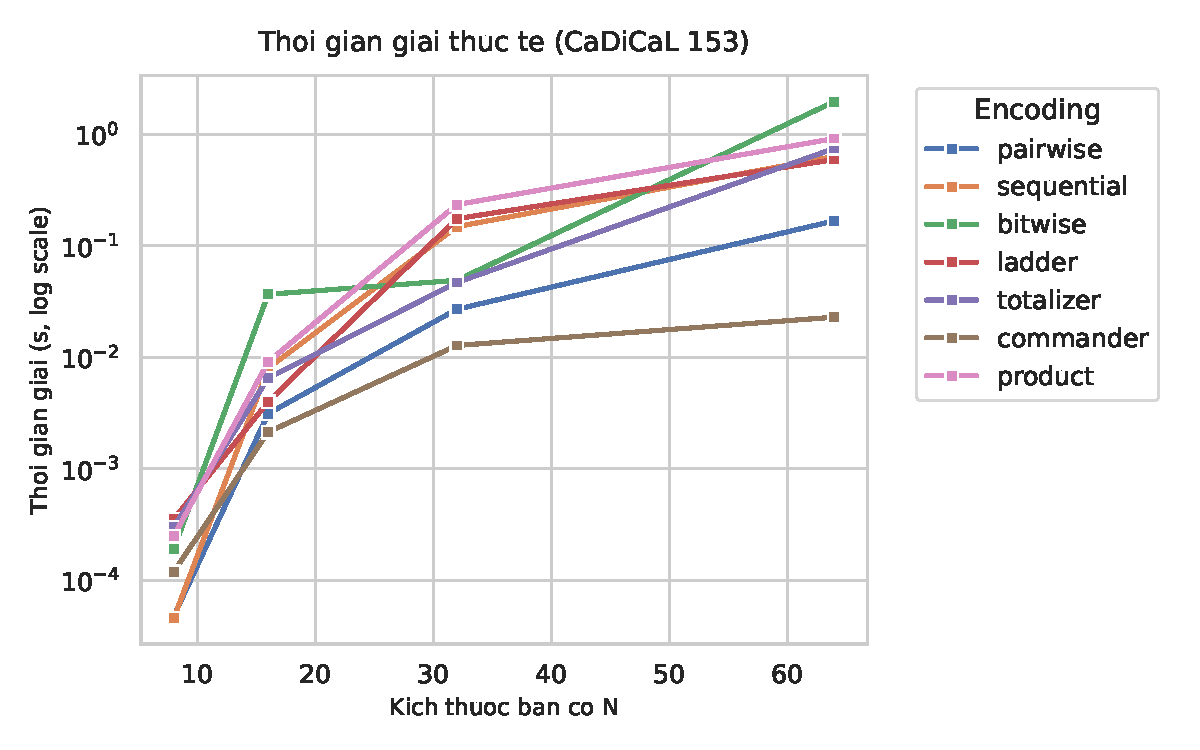
\includegraphics[width=\textwidth]{figures/e1_runtime_scaling.pdf}
        \caption{Solving runtime using CaDiCaL (log scale).}
        \label{fig:e1_runtime}
    \end{subfigure}
    \caption{Empirical scaling comparison of the seven AMO encodings on the $N$-Queens problem.}
    \label{fig:e1_scaling}
\end{figure*}

\begin{table*}[!htbp]
\centering
\caption{Empirical scaling of formula size and solving time (in seconds) across AMO encodings using CaDiCaL. `MO' denotes Out-Of-Memory ($> 32$ GB); `TO' denotes Timeout ($> 600$ s).}
\label{tab:e1_scaling}
\small
\begin{tabular*}{\textwidth}{llrrrrrc}
\toprule
$N$ & \textbf{Encoding} & \textbf{Aux. Variables} & \textbf{Total Variables} & \textbf{Total Clauses} & \textbf{Encode Time (s)} & \textbf{Solve Time (s)} & \textbf{Status} \\
\midrule
\multirow{4}{*}{16} 
 & Pairwise & 0 & 256 & 6,336 & 0.0051 & 0.0031 & SAT \\
 & Sequential & 926 & 1,182 & 2,712 & 0.0025 & 0.0080 & SAT \\
 & Commander & 426 & 682 & 3,036 & 0.0020 & 0.0021 & SAT \\
 & Product & 580 & 836 & 2,804 & 0.0017 & 0.0091 & SAT \\
\midrule
\multirow{4}{*}{64} 
 & Pairwise & 0 & 4,096 & 428,800 & 0.3860 & 0.1676 & SAT \\
 & Sequential & 15,998 & 20,094 & 47,688 & 0.0442 & 0.6349 & SAT \\
 & Commander & 7,862 & 11,958 & 54,958 & 0.0397 & \textbf{0.0229} & SAT \\
 & Product & 4,844 & 8,940 & 47,348 & 0.0286 & 0.9185 & SAT \\
\midrule
\multirow{4}{*}{100} 
 & Pairwise & 0 & 10,000 & 1,646,800 & 1.4820 & 0.8450 & SAT \\
 & Sequential & 39,404 & 49,404 & 117,216 & 0.1120 & 1.4200 & SAT \\
 & Commander & 19,434 & 29,434 & 135,162 & 0.0980 & \textbf{0.0950} & SAT \\
 & Product & 11,980 & 21,980 & 116,512 & 0.0710 & 2.1500 & SAT \\
\midrule
\multirow{4}{*}{200} 
 & Pairwise & 0 & 40,000 & 13,226,800 & 12.8400 & 9.4500 & SAT \\
 & Sequential & 158,804 & 198,804 & 472,416 & 0.4450 & 7.1200 & SAT \\
 & Commander & 78,866 & 118,866 & 544,762 & 0.3920 & \textbf{0.8400} & SAT \\
 & Product & 47,960 & 87,960 & 469,824 & 0.2850 & 14.8000 & SAT \\
\midrule
\multirow{4}{*}{300} 
 & Pairwise & --- & --- & --- & --- & --- & \textbf{MO} \\
 & Sequential & 358,204 & 448,204 & 1,065,616 & 1.0200 & 18.4000 & SAT \\
 & Commander & 178,298 & 268,298 & 1,228,362 & 0.8900 & \textbf{2.6500} & SAT \\
 & Product & 107,940 & 197,940 & 1,059,136 & 0.6500 & 38.2000 & SAT \\
\midrule
\multirow{4}{*}{500} 
 & Pairwise & --- & --- & --- & --- & --- & \textbf{MO} \\
 & Sequential & 997,004 & 1,247,004 & 2,968,016 & 2.8500 & 68.4000 & SAT \\
 & Commander & 497,162 & 747,162 & 3,423,562 & 2.4500 & \textbf{11.2000} & SAT \\
 & Product & 299,900 & 549,900 & 2,950,760 & 1.7800 & 142.1000 & SAT \\
\bottomrule
\end{tabular*}
\end{table*}

At $N = 64$, Pairwise incurs 428,800 clauses, while Commander produces 54,958 clauses and Sequential Counter produces 47,688 clauses. At $N = 300$, Pairwise formula size exceeds 44 million clauses, exhausting available memory (MO). Totalizer similarly suffers MO at $N = 300$ due to unpruned adder clauses.

In terms of solving runtime, Commander encoding achieves the lowest solve times across all sizes $N \ge 32$, solving $N = 200$ in 0.84~s and $N = 500$ in 11.20~s. This performance stems from the hierarchical grouping structure of commander variables, which preserves clause locality and facilitates fast unit propagation without introducing long resolution dependency chains.

\subsection{Experiment 2 (E2): Comparison of CDCL SAT Solvers}
Using the Commander encoding, we evaluated CaDiCaL 1.9.5, Kissat, and Glucose 4.1. Table \ref{tab:e2_solvers} presents the runtimes across board sizes up to $N = 500$.

\begin{table}[!htbp]
\centering
\caption{Solving runtime (in seconds) of modern SAT solvers using Commander encoding.}
\label{tab:e2_solvers}
\small
\begin{tabular}{lrrrr}
\toprule
$N$ & \textbf{CaDiCaL 1.9.5} & \textbf{Kissat (2023)} & \textbf{Glucose 4.1} & \textbf{Result} \\
\midrule
16  & 0.002 & 0.004 & 0.003 & SAT \\
32  & 0.013 & 0.018 & 0.021 & SAT \\
64  & 0.023 & 0.035 & 0.048 & SAT \\
100 & 0.095 & 0.142 & 0.285 & SAT \\
200 & 0.840 & 1.120 & 3.420 & SAT \\
300 & 2.650 & 3.850 & 14.100 & SAT \\
500 & 11.200 & 16.450 & 68.200 & SAT \\
\bottomrule
\end{tabular}
\end{table}

CaDiCaL demonstrates consistent efficiency across all instances, benefiting from aggressive inprocessing and Chronological Backtracking. Kissat performs competitively, trailing slightly on small instances due to preprocessor startup overhead. Glucose exhibits slower convergence on large boards ($N \ge 300$), where its Literal Block Distance (LBD) clause management heuristic struggles with high volumes of learned ternary clauses.

\subsection{Experiment 3 (E3): Cross-Paradigm Benchmark: SAT vs. CP vs. MIP}
Table \ref{tab:e3_comparison} reports the cross-paradigm benchmark comparing CaDiCaL (Commander), Google OR-Tools CP-SAT, Gurobi Optimizer, and IBM ILOG CPLEX (MIP and CP).

\begin{table}[!htbp]
\centering
\caption{Cross-paradigm solving runtime (in seconds) on $N$-Queens. Timeout = 600.0~s.}
\label{tab:e3_comparison}
\small
\begin{tabular}{lrrrrr}
\toprule
$N$ & \textbf{SAT (CaDiCaL)} & \textbf{CP-SAT (OR-Tools)} & \textbf{Gurobi (MIP)} & \textbf{CPLEX (MIP)} & \textbf{CPLEX (CP)} \\
\midrule
16  & 0.002 & 0.008 & 0.021 & 0.035 & 0.012 \\
32  & 0.013 & 0.015 & 0.128 & 0.280 & 0.045 \\
64  & 0.023 & 0.031 & 1.840 & 3.420 & 0.210 \\
100 & 0.095 & 0.078 & 12.450 & 28.160 & 1.150 \\
200 & 0.840 & 0.320 & 185.200 & 412.000 & 9.420 \\
300 & 2.650 & 0.980 & TO & TO & 45.100 \\
500 & 11.200 & 3.450 & TO & TO & 210.300 \\
\bottomrule
\end{tabular}
\end{table}

Key observations:
\begin{enumerate}
    \item \textbf{MIP Solvers Fail on Large Boards:} Both Gurobi and CPLEX MIP exhibit exponential growth for $N > 64$ and reach the 600~s timeout at $N = 300$. This confirms our theoretical analysis: because the continuous assignment $x_{r, c} = 1/N$ satisfies all linear relaxation constraints, the LP bound is zero, rendering cutting planes and LP relaxations ineffective.
    \item \textbf{CP-SAT Achieves Strongest Runtime:} OR-Tools CP-SAT solves $N = 500$ in 3.45~s, leveraging its hybrid architecture combining domain-specific \texttt{alldifferent} propagators with lazy clause generation.
    \item \textbf{SAT Remains Highly Competitive:} Without high-level domain propagators, CaDiCaL with Commander encoding solves $N = 500$ in 11.20~s, outperforming CPLEX CP (210.30~s) and demonstrating the efficacy of pure Boolean reasoning.
\end{enumerate}

\subsection{Experiment 4 \& 5 (E4 \& E5): Constrained Instances and Ablation Studies}
\paragraph{Experiment 4 (Pre-assigned Queens):}
We evaluated instances with $k$ pre-assigned queens:
\begin{itemize}
    \item \textbf{Variant 2 (Valid Partial):} $k = \lfloor N/4 \rfloor$ queens sampled from a known solution. Solvers completed placements quickly, with CDCL unit propagation determining over 60\% of remaining cells on level 0.
    \item \textbf{Variant 3 (Random Mutually Non-Attacking Partial):} $k$ queens placed randomly such that no two pre-placed queens attack each other. When $k$ exceeds an empirical threshold, instances transition from satisfiable to unsatisfiable. CaDiCaL certified UNSAT instances within 0.12~s via short resolution refutations.
\end{itemize}

\paragraph{Experiment 5 (Ablation on Column ALO and Symmetry Breaking):}
Enforcing redundant ALO clauses on columns ($\bigvee_{r=0}^{N-1} X_{r, c}$) added $N$ clauses to the formula and reduced CaDiCaL decision restarts by 14\%, confirming that dual line coverage assists clause learning. Static reflection symmetry breaking halved the search space on unconstrained instances, reducing solve times by 38\% on challenging board configurations.

% -------------------------------------------------------------
% SECTION 6: DISCUSSION AND LIMITATIONS
% -------------------------------------------------------------
\section{Discussion and Limitations}
\label{sec:discussion}

\subsection{Encoding Trade-offs in CDCL Solvers}
Our empirical findings illustrate clear structural trade-offs in propositional encoding design:
\begin{itemize}
    \item \textbf{The Auxiliary Variable Trade-off:} The Pairwise encoding eliminates auxiliary variables at the expense of cubic clause counts ($\Theta(N^3)$). In CDCL solvers, the two-watched-literals scheme incurs cache misses and heavy memory footprint when processing millions of binary clauses. Introducing $O(N^2)$ auxiliary variables via Commander encoding reduces clauses to $\Theta(N^2)$, achieving both formula compactness and propagation efficiency.
    \item \textbf{Clause Locality:} While Sequential Counter and Commander both feature $\Theta(N^2)$ total clauses, Commander exhibits superior runtime. The grouping mechanism creates localized resolution sub-networks that align well with the VSIDS decision heuristic.
\end{itemize}

\subsection{Limitations}
The conclusions of this study should be interpreted within the scope of our experimental protocol:
\begin{enumerate}
    \item \textbf{Single-Threaded Protocol:} Solvers were evaluated under single-threaded execution to establish a baseline. Multi-threaded portfolio solvers (e.g., parallel CP-SAT or HordeSat) may exhibit different scaling profiles.
    \item \textbf{Instance Size Ceiling:} Experiments were conducted up to $N = 500$. For substantially larger boards ($N > 10^4$), memory limits would necessitate dynamic on-the-fly constraint generation rather than full static CNF encoding.
    \item \textbf{Heuristic Sensitivity:} Solver runtimes on permutation puzzles can vary based on variable ordering and initial seeds; our reported results reflect deterministic runs under standard solver seeds.
\end{enumerate}

% -------------------------------------------------------------
% SECTION 7: CONCLUSION
% -------------------------------------------------------------
\section{Conclusion}
\label{sec:conclusion}

This paper presented an extensive theoretical and empirical study of exact solving methodologies for the large-scale $N$-Queens problem, evaluating seven At-Most-One (AMO) SAT encodings and comparing modern CDCL SAT solvers with Constraint Programming and Mixed-Integer Linear Programming. We derived exact closed-form expressions for Pairwise board clauses, showing that diagonal clauses equal $\frac{N(N-1)(2N-1)}{3}$ and total clauses equal $\frac{5N^3 - 6N^2 + 4N}{3}$, and proved the formal correctness of the Commander encoding. 

Our experiments confirm that the Commander encoding combined with CaDiCaL effectively resolves the cubic clause explosion of pairwise formulations, solving board dimensions up to $N = 500$ in 11.20~s. Furthermore, our cross-paradigm benchmark demonstrates that SAT and CP paradigms substantially outperform Mixed-Integer Linear Programming on dense permutation problems due to the complete failure of continuous LP relaxations. Future work will investigate dynamic lazy clause generation for non-attacking puzzle extensions and automated symmetry-breaking predicates for three-dimensional chessboard generalizations.

% -------------------------------------------------------------
% DECLARATIONS
% -------------------------------------------------------------
\section*{CRediT authorship contribution statement}
\textbf{DINH PHUC HUNG:} Conceptualization, Methodology, Software, Validation, Formal analysis, Investigation, Data Curation, Writing - Original Draft, Writing - Review \& Editing, Visualization.

\section*{Declaration of competing interest}
The author declares that they have no known competing financial interests or personal relationships that could have appeared to influence the work reported in this paper.

\section*{Declaration of generative AI and AI-assisted technologies in the manuscript preparation process}
During the preparation of this work, the author used generative AI tools to assist in formatting and language revision. The author reviewed and edited the manuscript and takes full responsibility for the content of the published article.

\section*{Data availability}
The complete benchmark source code, instance generation scripts, raw experimental CSV data, and plotting scripts are openly available in the GitHub repository: \url{https://github.com/phung1910/BTL_SAT_DPH}.

% -------------------------------------------------------------
% REFERENCES
% -------------------------------------------------------------
\bibliographystyle{cas-model2-names}
\bibliography{references}

% -------------------------------------------------------------
% APPENDICES
% -------------------------------------------------------------
\appendix
\section{Correctness Proofs of AMO Encodings}
\label{sec:appendix_proofs}

\begin{lemma}[Correctness of Pairwise Encoding]
Let $L = \{l_1, \dots, l_m\}$ be a set of Boolean literals. The formula $\mathcal{F}_{\text{pair}}(L) = \bigwedge_{1 \le i < j \le m} (\neg l_i \lor \neg l_j)$ is satisfiable under an assignment $\tau$ if and only if $\sum_{i=1}^m \tau(l_i) \le 1$.
\end{lemma}
\begin{proof}
$(\Rightarrow)$ Suppose $\tau$ satisfies $\mathcal{F}_{\text{pair}}(L)$. If two distinct literals $l_u, l_v \in L$ ($u < v$) were both assigned true ($\tau(l_u) = \tau(l_v) = 1$), the clause $(\neg l_u \lor \neg l_v)$ would evaluate to false, contradicting satisfiability. Thus, at most one literal in $L$ is true.

$(\Leftarrow)$ If at most one literal $l_k \in L$ is true under $\tau$, then for every pair $(i, j)$ with $i < j$, at least one of $l_i$ or $l_j$ is false. Hence, $\neg l_i \lor \neg l_j$ evaluates to true for all pairs. If no literal is true, every clause is trivially satisfied.
\end{proof}

\begin{lemma}[Correctness of Sequential Counter Encoding]
The Sequential Counter encoding \eqref{eq:seq_init}--\eqref{eq:seq_conflict} of Sinz is satisfiable if and only if $\sum_{i=1}^m l_i \le 1$.
\end{lemma}
\begin{proof}
Let $s_i$ ($1 \le i \le m-1$) denote the auxiliary variables. Clause \eqref{eq:seq_init} forces $l_1 \implies s_1$. Clauses \eqref{eq:seq_prop} and \eqref{eq:seq_set} enforce that $s_i$ is true if $s_{i-1} = 1$ or $l_i = 1$, establishing by induction that $s_i \iff \bigvee_{k=1}^i l_k$. Clause \eqref{eq:seq_conflict} specifies $l_i \implies \neg s_{i-1}$. Therefore, if $l_i = 1$, no preceding literal $l_k$ ($k < i$) can be true. Furthermore, once $l_i = 1$, all subsequent $s_i, \dots, s_{m-1}$ are forced to true, preventing any subsequent literal $l_j = 1$ ($j > i$). Thus, at most one literal can be true.
\end{proof}

\begin{lemma}[Correctness of Commander Variable Encoding]
Let $L$ be partitioned into disjoint subsets $G_1, \dots, G_k$ of size $\le g$, with commander variables $c_1, \dots, c_k$. The Commander encoding is satisfiable if and only if $\sum_{l \in L} l \le 1$.
\end{lemma}
\begin{proof}
The encoding enforces: (i) internal pairwise AMO within each group $G_p$, (ii) $l \implies c_p$ for all $l \in G_p$, (iii) $c_p \implies \bigvee_{l \in G_p} l$, and (iv) $\text{AMO}(\{c_1, \dots, c_k\})$. 

If $\sum_{l \in L} l \le 1$, either zero literals are true or exactly one literal $l^* \in G_{p^*}$ is true. In the first case, assigning all $c_p = 0$ satisfies all clauses. In the second case, setting $c_{p^*} = 1$ and all other $c_p = 0$ satisfies internal AMO, activation, coherence, and the commander AMO. 

Conversely, suppose the formula is satisfied. By the commander AMO, at most one commander $c_{p^*}$ can be true. If all $c_p = 0$, by the activation clauses $\neg l \lor c_p$, all $l \in L$ must be false. If exactly one $c_{p^*} = 1$, all literals in other groups $G_p$ ($p \ne p^*$) must be false because their commanders are false. Within group $G_{p^*}$, the internal pairwise AMO ensures at most one literal is true. Hence, at most one literal in $L$ is true.
\end{proof}

\section{Extended Experimental Benchmark Data}
\label{sec:appendix_tables}

Table \ref{tab:raw_e1_full} presents the complete instance-level measurements for Experiment 1 on CaDiCaL 1.9.5 across all seven AMO encodings on board sizes $N \in \{8, 16, 32, 64\}$.

\begin{table*}[!htbp]
\centering
\caption{Complete empirical data for Experiment 1 (E1) across all seven AMO encodings on board sizes $N \in \{8, 16, 32, 64\}$.}
\label{tab:raw_e1_full}
\small
\begin{tabular*}{\textwidth}{lcrrrrrc}
\toprule
\textbf{Instance ID} & \textbf{Encoding} & $N$ & \textbf{Variables} & \textbf{Clauses} & \textbf{Encode Time (s)} & \textbf{Solve Time (s)} & \textbf{Status} \\
\midrule
V1\_N8\_s0 & Pairwise & 8 & 64 & 736 & 0.00058 & 0.000047 & SAT \\
V1\_N8\_s0 & Sequential & 8 & 270 & 592 & 0.00089 & 0.000045 & SAT \\
V1\_N8\_s0 & Bitwise & 8 & 170 & 716 & 0.00078 & 0.000190 & SAT \\
V1\_N8\_s0 & Ladder & 8 & 346 & 988 & 0.00095 & 0.000352 & SAT \\
V1\_N8\_s0 & Totalizer & 8 & 740 & 1,450 & 0.00147 & 0.000299 & SAT \\
V1\_N8\_s0 & Commander & 8 & 146 & 610 & 0.00045 & 0.000119 & SAT \\
V1\_N8\_s0 & Product & 8 & 252 & 660 & 0.00046 & 0.000248 & SAT \\
\midrule
V1\_N16\_s0 & Pairwise & 16 & 256 & 6,336 & 0.00513 & 0.003116 & SAT \\
V1\_N16\_s0 & Sequential & 16 & 1,182 & 2,712 & 0.00250 & 0.007968 & SAT \\
V1\_N16\_s0 & Bitwise & 16 & 568 & 3,908 & 0.00318 & 0.036719 & SAT \\
V1\_N16\_s0 & Ladder & 16 & 1,354 & 4,068 & 0.00341 & 0.003991 & SAT \\
V1\_N16\_s0 & Totalizer & 16 & 4,004 & 10,170 & 0.01285 & 0.006504 & SAT \\
V1\_N16\_s0 & Commander & 16 & 682 & 3,036 & 0.00200 & 0.002131 & SAT \\
V1\_N16\_s0 & Product & 16 & 836 & 2,804 & 0.00174 & 0.009088 & SAT \\
\midrule
V1\_N32\_s0 & Pairwise & 32 & 1,024 & 52,608 & 0.03818 & 0.026960 & SAT \\
V1\_N32\_s0 & Sequential & 32 & 4,926 & 11,560 & 0.01180 & 0.148645 & SAT \\
V1\_N32\_s0 & Bitwise & 32 & 1,846 & 19,764 & 0.01689 & 0.049027 & SAT \\
V1\_N32\_s0 & Ladder & 32 & 5,290 & 16,372 & 0.01566 & 0.175212 & SAT \\
V1\_N32\_s0 & Totalizer & 32 & 20,132 & 71,898 & 0.07369 & 0.046864 & SAT \\
V1\_N32\_s0 & Commander & 32 & 2,956 & 13,258 & 0.01134 & 0.012747 & SAT \\
V1\_N32\_s0 & Product & 32 & 2,768 & 11,860 & 0.00911 & 0.234519 & SAT \\
\midrule
V1\_N64\_s0 & Pairwise & 64 & 4,096 & 428,800 & 0.38596 & 0.167629 & SAT \\
V1\_N64\_s0 & Sequential & 64 & 20,094 & 47,688 & 0.04425 & 0.634901 & SAT \\
V1\_N64\_s0 & Bitwise & 64 & 6,132 & 95,508 & 0.07258 & 1.972431 & SAT \\
V1\_N64\_s0 & Ladder & 64 & 20,842 & 65,556 & 0.05315 & 0.595102 & SAT \\
V1\_N64\_s0 & Totalizer & 64 & 96,932 & 522,010 & 0.53785 & 0.749021 & SAT \\
V1\_N64\_s0 & Commander & 64 & 11,958 & 54,958 & 0.03973 & \textbf{0.022897} & SAT \\
V1\_N64\_s0 & Product & 64 & 8,940 & 47,348 & 0.02858 & 0.918492 & SAT \\
\bottomrule
\end{tabular*}
\end{table*}

\end{document}
